\let\negmedspace\undefined
\let\negthickspace\undefined
\documentclass[journal]{IEEEtran}
\usepackage[a5paper, margin=10mm, onecolumn]{geometry}
%\usepackage{lmodern} % Ensure lmodern is loaded for pdflatex
\usepackage{tfrupee} % Include tfrupee package

\setlength{\headheight}{1cm} % Set the height of the header box
\setlength{\headsep}{0mm}     % Set the distance between the header box and the top of the text

\usepackage{gvv-book}
\usepackage{gvv}
\usepackage{cite}
\usepackage{amsmath,amssymb,amsfonts,amsthm}
\usepackage{algorithmic}
\usepackage{graphicx}
\usepackage{textcomp}
\usepackage{xcolor}
\usepackage{txfonts}
\usepackage{listings}
\usepackage{enumitem}
\usepackage{mathtools}
\usepackage{gensymb}
\usepackage{comment}
\usepackage[breaklinks=true]{hyperref}
\usepackage{tkz-euclide} 
\usepackage{listings}
% \usepackage{gvv}                                        
\def\inputGnumericTable{}                                 
\usepackage[latin1]{inputenc}                                
\usepackage{color}                                            
\usepackage{array}                                            
\usepackage{longtable}                                       
\usepackage{calc}                                             
\usepackage{multirow}                                         
\usepackage{hhline}                                           
\usepackage{ifthen}                                           
\usepackage{lscape}
\begin{document}

\bibliographystyle{IEEEtran}
\vspace{3cm}

\title{1.1.9.23}
\author{AI24BTECH11022 - Pabbuleti Venkata Charan Teja}
\maketitle

\renewcommand{\thefigure}{\theenumi}
\renewcommand{\thetable}{\theenumi}

\textbf{Question:}\\
If the point $P\myvec{0\\2\\}$ is equidistant from the points $Q\myvec{3\\k\\}$ and $R\myvec{k\\5\\}$, find the value of k.

\hfill{(10, 2018)}

\textbf{Solution:}

\begin{table}[h!]
\renewcommand{\thetable}{1}
    \centering
   \begin{tabular}{|c| c |}
\hline
\textbf{Variable} & \textbf{Value} \\
\hline
$A$ & \myvec{1 \\ -5\\}\\
\hline
$B$ & \myvec{-4 \\ 5\\}\\
\hline
$k:1$    & Ratio in which the line $AB$ is divided by $x$-axis \\
\hline
$X$  & Point of division of $A$ , $B$\\
\hline
\end{tabular} 
   \def\tablename{Table}
   \caption{Variables Used}
    \label{tab1.1.5.10.1}
\end{table}

If $P$ is equidistant from the points $Q$ and $R$,
\begin{align}
    \abs{\abs{P-Q}}&=\abs{\abs{P-R}}\label{eq1.1.9.23.1}\\
    \implies\abs{\abs{P-Q}}^{2}&=\abs{\abs{P-R}}^{2}\label{eq1.1.9.23.2}\\
\implies\abs{\abs{P}}^{2}-2P^{\top}Q+\abs{\abs{Q}}^{2}&=\abs{\abs{P}}^{2}-2P^{\top}R+\abs{\abs{R}}^{2}\label{eq1.1.9.23.3}
\end{align}

which can be simplified to obtain,
\begin{align}
    \brak{Q-R}^{\top}P&=\frac{\abs{\abs{Q}}^{2}-\abs{\abs{R}}^{2}}{2}\label{eq1.1.9.23.4}\\
   \brak{Q-R}^{\top}&=\myvec{3-k\\k-5\\}\label{eq1.1.9.23.5}\\
   \brak{Q-R}^{\top}P&=\myvec{3-k && k-5}\myvec{0\\2\\}\label{eq1.1.9.23.6}\\
   \brak{Q-R}^{\top}P&=2k-10\label{eq1.1.9.23.7}\\
    \abs{\abs{Q}}^{2}=Q^{\top}Q&=9+k^{2}\label{eq1.1.9.23.8}\\
    \abs{\abs{R}}^{2}=R^{\top}R&=25+k^{2}\label{eq1.1.9.23.9}\\
    \frac{\abs{\abs{Q}}^{2}-\abs{\abs{R}}^{2}}{2}&=-8\label{eq1.1.9.23.10}
\end{align}

Substituting the equations gives,
\begin{align}
    2k-10&=-8\label{eq1.1.9.23.11}\\
    \implies k&=1\label{eq1.1.9.23.12}
\end{align}

$\therefore$The points $Q$ and $R$ are,
\begin{align}
    Q&=\myvec{3\\1\\}\label{eq1.1.9.23.13}\\
    R&=\myvec{1\\5\\}\label{eq1.1.9.23.14}
\end{align}


\begin{figure}[h!]
\renewcommand{\thefigure}{1}
    \centering
    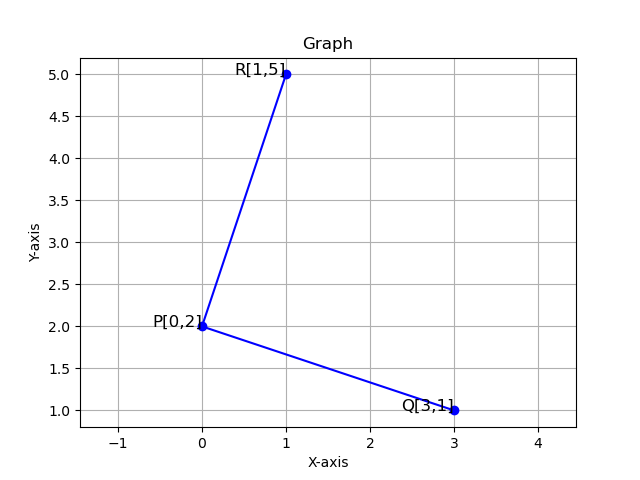
\includegraphics[width=0.7\linewidth]{figs/plot.png}
    \caption{Plot of the points}
    \label{fig1.1.5.10.1}
\end{figure}

\end{document}